\PassOptionsToPackage{unicode=true}{hyperref} % options for packages loaded elsewhere
\PassOptionsToPackage{hyphens}{url}
%
\documentclass[]{article}
\usepackage{lmodern}
\usepackage{amssymb,amsmath}
\usepackage{ifxetex,ifluatex}
\usepackage{fixltx2e} % provides \textsubscript
\ifnum 0\ifxetex 1\fi\ifluatex 1\fi=0 % if pdftex
  \usepackage[T1]{fontenc}
  \usepackage[utf8]{inputenc}
  \usepackage{textcomp} % provides euro and other symbols
\else % if luatex or xelatex
  \usepackage{unicode-math}
  \defaultfontfeatures{Ligatures=TeX,Scale=MatchLowercase}
\fi
% use upquote if available, for straight quotes in verbatim environments
\IfFileExists{upquote.sty}{\usepackage{upquote}}{}
% use microtype if available
\IfFileExists{microtype.sty}{%
\usepackage[]{microtype}
\UseMicrotypeSet[protrusion]{basicmath} % disable protrusion for tt fonts
}{}
\IfFileExists{parskip.sty}{%
\usepackage{parskip}
}{% else
\setlength{\parindent}{0pt}
\setlength{\parskip}{6pt plus 2pt minus 1pt}
}
\usepackage{hyperref}
\hypersetup{
            pdftitle={Bagging and Boosting Linear Models for Regression},
            pdfauthor={Shan Chen},
            pdfborder={0 0 0},
            breaklinks=true}
\urlstyle{same}  % don't use monospace font for urls
\usepackage[margin=1in]{geometry}
\usepackage{color}
\usepackage{fancyvrb}
\newcommand{\VerbBar}{|}
\newcommand{\VERB}{\Verb[commandchars=\\\{\}]}
\DefineVerbatimEnvironment{Highlighting}{Verbatim}{commandchars=\\\{\}}
% Add ',fontsize=\small' for more characters per line
\usepackage{framed}
\definecolor{shadecolor}{RGB}{248,248,248}
\newenvironment{Shaded}{\begin{snugshade}}{\end{snugshade}}
\newcommand{\AlertTok}[1]{\textcolor[rgb]{0.94,0.16,0.16}{#1}}
\newcommand{\AnnotationTok}[1]{\textcolor[rgb]{0.56,0.35,0.01}{\textbf{\textit{#1}}}}
\newcommand{\AttributeTok}[1]{\textcolor[rgb]{0.77,0.63,0.00}{#1}}
\newcommand{\BaseNTok}[1]{\textcolor[rgb]{0.00,0.00,0.81}{#1}}
\newcommand{\BuiltInTok}[1]{#1}
\newcommand{\CharTok}[1]{\textcolor[rgb]{0.31,0.60,0.02}{#1}}
\newcommand{\CommentTok}[1]{\textcolor[rgb]{0.56,0.35,0.01}{\textit{#1}}}
\newcommand{\CommentVarTok}[1]{\textcolor[rgb]{0.56,0.35,0.01}{\textbf{\textit{#1}}}}
\newcommand{\ConstantTok}[1]{\textcolor[rgb]{0.00,0.00,0.00}{#1}}
\newcommand{\ControlFlowTok}[1]{\textcolor[rgb]{0.13,0.29,0.53}{\textbf{#1}}}
\newcommand{\DataTypeTok}[1]{\textcolor[rgb]{0.13,0.29,0.53}{#1}}
\newcommand{\DecValTok}[1]{\textcolor[rgb]{0.00,0.00,0.81}{#1}}
\newcommand{\DocumentationTok}[1]{\textcolor[rgb]{0.56,0.35,0.01}{\textbf{\textit{#1}}}}
\newcommand{\ErrorTok}[1]{\textcolor[rgb]{0.64,0.00,0.00}{\textbf{#1}}}
\newcommand{\ExtensionTok}[1]{#1}
\newcommand{\FloatTok}[1]{\textcolor[rgb]{0.00,0.00,0.81}{#1}}
\newcommand{\FunctionTok}[1]{\textcolor[rgb]{0.00,0.00,0.00}{#1}}
\newcommand{\ImportTok}[1]{#1}
\newcommand{\InformationTok}[1]{\textcolor[rgb]{0.56,0.35,0.01}{\textbf{\textit{#1}}}}
\newcommand{\KeywordTok}[1]{\textcolor[rgb]{0.13,0.29,0.53}{\textbf{#1}}}
\newcommand{\NormalTok}[1]{#1}
\newcommand{\OperatorTok}[1]{\textcolor[rgb]{0.81,0.36,0.00}{\textbf{#1}}}
\newcommand{\OtherTok}[1]{\textcolor[rgb]{0.56,0.35,0.01}{#1}}
\newcommand{\PreprocessorTok}[1]{\textcolor[rgb]{0.56,0.35,0.01}{\textit{#1}}}
\newcommand{\RegionMarkerTok}[1]{#1}
\newcommand{\SpecialCharTok}[1]{\textcolor[rgb]{0.00,0.00,0.00}{#1}}
\newcommand{\SpecialStringTok}[1]{\textcolor[rgb]{0.31,0.60,0.02}{#1}}
\newcommand{\StringTok}[1]{\textcolor[rgb]{0.31,0.60,0.02}{#1}}
\newcommand{\VariableTok}[1]{\textcolor[rgb]{0.00,0.00,0.00}{#1}}
\newcommand{\VerbatimStringTok}[1]{\textcolor[rgb]{0.31,0.60,0.02}{#1}}
\newcommand{\WarningTok}[1]{\textcolor[rgb]{0.56,0.35,0.01}{\textbf{\textit{#1}}}}
\usepackage{graphicx,grffile}
\makeatletter
\def\maxwidth{\ifdim\Gin@nat@width>\linewidth\linewidth\else\Gin@nat@width\fi}
\def\maxheight{\ifdim\Gin@nat@height>\textheight\textheight\else\Gin@nat@height\fi}
\makeatother
% Scale images if necessary, so that they will not overflow the page
% margins by default, and it is still possible to overwrite the defaults
% using explicit options in \includegraphics[width, height, ...]{}
\setkeys{Gin}{width=\maxwidth,height=\maxheight,keepaspectratio}
\setlength{\emergencystretch}{3em}  % prevent overfull lines
\providecommand{\tightlist}{%
  \setlength{\itemsep}{0pt}\setlength{\parskip}{0pt}}
\setcounter{secnumdepth}{0}
% Redefines (sub)paragraphs to behave more like sections
\ifx\paragraph\undefined\else
\let\oldparagraph\paragraph
\renewcommand{\paragraph}[1]{\oldparagraph{#1}\mbox{}}
\fi
\ifx\subparagraph\undefined\else
\let\oldsubparagraph\subparagraph
\renewcommand{\subparagraph}[1]{\oldsubparagraph{#1}\mbox{}}
\fi

% set default figure placement to htbp
\makeatletter
\def\fps@figure{htbp}
\makeatother


\title{Bagging and Boosting Linear Models for Regression}
\author{Shan Chen}
\date{4/27/2020}

\begin{document}
\maketitle

\#setup

\begin{Shaded}
\begin{Highlighting}[]
\KeywordTok{library}\NormalTok{(tidyverse)}
\KeywordTok{library}\NormalTok{(randomForest)}
\end{Highlighting}
\end{Shaded}

\begin{verbatim}
## randomForest 4.6-14
\end{verbatim}

\begin{verbatim}
## Type rfNews() to see new features/changes/bug fixes.
\end{verbatim}

\begin{verbatim}
## 
## Attaching package: 'randomForest'
\end{verbatim}

\begin{verbatim}
## The following object is masked from 'package:dplyr':
## 
##     combine
\end{verbatim}

\begin{verbatim}
## The following object is masked from 'package:ggplot2':
## 
##     margin
\end{verbatim}

\begin{Shaded}
\begin{Highlighting}[]
\KeywordTok{library}\NormalTok{(glmnet)}
\end{Highlighting}
\end{Shaded}

\begin{verbatim}
## Loading required package: Matrix
\end{verbatim}

\begin{verbatim}
## 
## Attaching package: 'Matrix'
\end{verbatim}

\begin{verbatim}
## The following objects are masked from 'package:tidyr':
## 
##     expand, pack, unpack
\end{verbatim}

\begin{verbatim}
## Loaded glmnet 3.0-2
\end{verbatim}

\begin{Shaded}
\begin{Highlighting}[]
\KeywordTok{library}\NormalTok{(gbm)}
\end{Highlighting}
\end{Shaded}

\begin{verbatim}
## Loaded gbm 2.1.5
\end{verbatim}

\begin{Shaded}
\begin{Highlighting}[]
\KeywordTok{library}\NormalTok{(tidyverse)}
\KeywordTok{library}\NormalTok{(tree)}
\end{Highlighting}
\end{Shaded}

\begin{verbatim}
## Registered S3 method overwritten by 'tree':
##   method     from
##   print.tree cli
\end{verbatim}

1:

\begin{Shaded}
\begin{Highlighting}[]
\NormalTok{dataDir <-}\StringTok{ "/Users/shawnchen/Desktop/rzhw"}
\NormalTok{dataFile <-}\StringTok{ "CountyElection.csv"}
\NormalTok{dictFile <-}\StringTok{ "County_Facts_Dictionary.csv"}

\NormalTok{countyElection.df <-}\StringTok{ }\KeywordTok{read.csv}\NormalTok{(}\KeywordTok{file.path}\NormalTok{(dataDir,dataFile))}
\KeywordTok{names}\NormalTok{(countyElection.df)}
\end{Highlighting}
\end{Shaded}

\begin{verbatim}
##  [1] "fips"      "PST045214" "AGE135214" "AGE295214" "AGE775214" "SEX255214"
##  [7] "RHI125214" "RHI225214" "RHI325214" "RHI425214" "RHI525214" "RHI625214"
## [13] "RHI725214" "RHI825214" "POP715213" "POP645213" "POP815213" "EDU635213"
## [19] "EDU685213" "VET605213" "LFE305213" "HSG010214" "HSG445213" "HSG096213"
## [25] "HSG495213" "HSD410213" "HSD310213" "INC910213" "INC110213" "PVY020213"
## [31] "BZA010213" "BZA110213" "BZA115213" "NES010213" "SBO001207" "SBO315207"
## [37] "SBO115207" "SBO215207" "SBO515207" "SBO415207" "SBO015207" "MAN450207"
## [43] "WTN220207" "RTN131207" "AFN120207" "BPS030214" "POP060210" "State"    
## [49] "VoterProp"
\end{verbatim}

\begin{Shaded}
\begin{Highlighting}[]
\NormalTok{dictionary.df <-}\KeywordTok{read.csv}\NormalTok{(}\KeywordTok{file.path}\NormalTok{(dataDir,dictFile))}
\KeywordTok{dim}\NormalTok{(countyElection.df)}
\end{Highlighting}
\end{Shaded}

\begin{verbatim}
## [1] 2711   49
\end{verbatim}

\begin{Shaded}
\begin{Highlighting}[]
\NormalTok{countyIDInfo.df <-}\StringTok{ }\NormalTok{countyElection.df }\OperatorTok\StringTok{ }
\StringTok{  }\KeywordTok{select}\NormalTok{(fips,State)}

\NormalTok{countyElection.df <-}\StringTok{ }\NormalTok{countyElection.df }\OperatorTok\StringTok{ }
\StringTok{  }\KeywordTok{select}\NormalTok{(}\OperatorTok{-}\NormalTok{fips,}\OperatorTok{-}\NormalTok{State)}

\NormalTok{dictionary.df <-}\StringTok{ }\NormalTok{dictionary.df }\OperatorTok\StringTok{ }
\StringTok{  }\KeywordTok{filter}\NormalTok{(}\OperatorTok{!}\StringTok{ }\NormalTok{column_name }\OperatorTok\StringTok{ }\KeywordTok{c}\NormalTok{(}\StringTok{"fips"}\NormalTok{,}\StringTok{"State"}\NormalTok{))}
\end{Highlighting}
\end{Shaded}

Random Forest

\begin{Shaded}
\begin{Highlighting}[]
\NormalTok{N <-}\StringTok{ }\KeywordTok{nrow}\NormalTok{(countyElection.df)}
\NormalTok{n <-}\StringTok{ }\DecValTok{500}
\NormalTok{build <-}\StringTok{ }\KeywordTok{sample}\NormalTok{(}\DecValTok{1}\OperatorTok{:}\NormalTok{N,n,}\DataTypeTok{rep=}\NormalTok{F) }
\NormalTok{data.df <-}\StringTok{ }\NormalTok{countyElection.df[build,]}
\NormalTok{numTree <-}\StringTok{ }\DecValTok{100}
\NormalTok{numPred <-}\StringTok{ }\DecValTok{45}
\NormalTok{mod.rf <-}\StringTok{ }\KeywordTok{randomForest}\NormalTok{(VoterProp }\OperatorTok{~}\NormalTok{.,}
                        \DataTypeTok{data=}\NormalTok{data.df, }
                        \DataTypeTok{ntree=}\NormalTok{numTree, }
                        \DataTypeTok{mtry=}\NormalTok{numPred}\OperatorTok{/}\DecValTok{3}\NormalTok{)}
\NormalTok{mod.rf}
\end{Highlighting}
\end{Shaded}

\begin{verbatim}
## 
## Call:
##  randomForest(formula = VoterProp ~ ., data = data.df, ntree = numTree,      mtry = numPred/3) 
##                Type of random forest: regression
##                      Number of trees: 100
## No. of variables tried at each split: 15
## 
##           Mean of squared residuals: 0.003579648
##                     % Var explained: 62.77
\end{verbatim}

\begin{Shaded}
\begin{Highlighting}[]
\KeywordTok{plot}\NormalTok{(mod.rf)}
\end{Highlighting}
\end{Shaded}

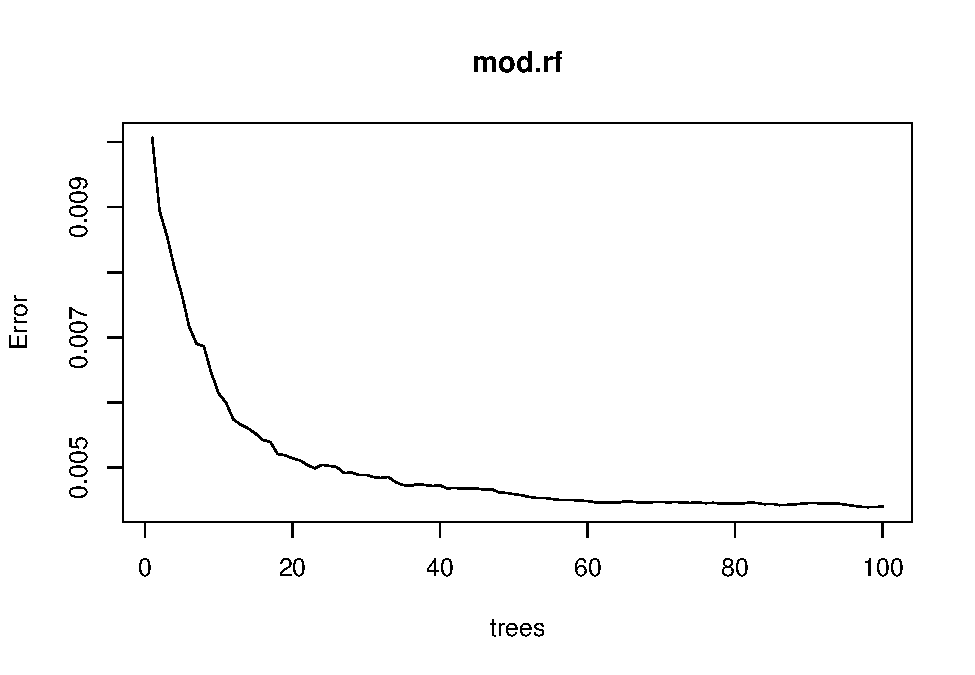
\includegraphics{4271_files/figure-latex/unnamed-chunk-3-1.pdf} Bagging

\begin{Shaded}
\begin{Highlighting}[]
\NormalTok{n <-}\StringTok{ }\DecValTok{500}
\NormalTok{build <-}\StringTok{ }\KeywordTok{sample}\NormalTok{(}\DecValTok{1}\OperatorTok{:}\NormalTok{N,n,}\DataTypeTok{rep=}\NormalTok{F)}
\NormalTok{data.df <-}\StringTok{ }\NormalTok{countyElection.df[build,]}
\CommentTok{##Data to test/validate the model}
\NormalTok{n <-}\StringTok{ }\DecValTok{500}
\NormalTok{test <-}\StringTok{ }\KeywordTok{sample}\NormalTok{(}\KeywordTok{setdiff}\NormalTok{(}\DecValTok{1}\OperatorTok{:}\NormalTok{N,build),n,}\DataTypeTok{rep=}\NormalTok{F)}
\NormalTok{test.df <-}\StringTok{ }\NormalTok{countyElection.df[test,]}
\NormalTok{numTree <-}\StringTok{ }\DecValTok{100}
\NormalTok{numPred <-}\StringTok{ }\DecValTok{45}
\NormalTok{mod.bag <-}\StringTok{ }\KeywordTok{randomForest}\NormalTok{(VoterProp }\OperatorTok{~}\NormalTok{.,}
                        \DataTypeTok{data=}\NormalTok{data.df, }
                        \DataTypeTok{ntree=}\NormalTok{numTree, }
                        \DataTypeTok{mtry=}\NormalTok{numPred)}
\NormalTok{mod.bag}
\end{Highlighting}
\end{Shaded}

\begin{verbatim}
## 
## Call:
##  randomForest(formula = VoterProp ~ ., data = data.df, ntree = numTree,      mtry = numPred) 
##                Type of random forest: regression
##                      Number of trees: 100
## No. of variables tried at each split: 45
## 
##           Mean of squared residuals: 0.004194657
##                     % Var explained: 58.95
\end{verbatim}

\begin{Shaded}
\begin{Highlighting}[]
\KeywordTok{plot}\NormalTok{(mod.bag)}
\end{Highlighting}
\end{Shaded}

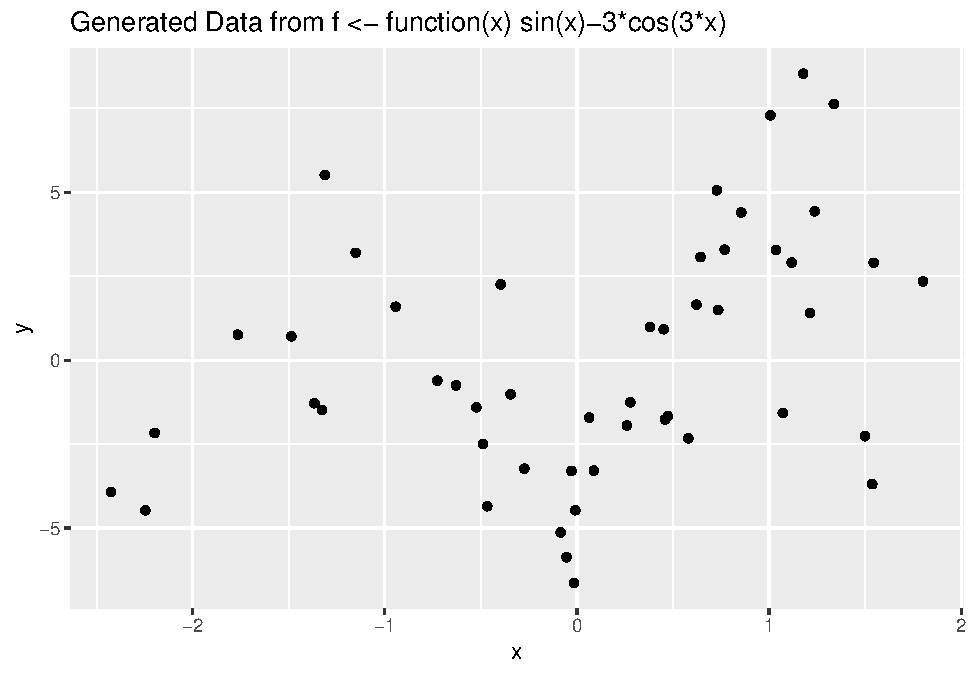
\includegraphics{4271_files/figure-latex/unnamed-chunk-4-1.pdf}
boosting:

\begin{Shaded}
\begin{Highlighting}[]
\NormalTok{numPreds <-}\StringTok{ }\KeywordTok{ncol}\NormalTok{(countyElection.df)}\OperatorTok{-}\DecValTok{1}
\NormalTok{numTrees <-}\StringTok{ }\DecValTok{800}
\NormalTok{theShrinkage <-}\StringTok{ }\FloatTok{0.1}
\NormalTok{theDepth <-}\StringTok{ }\DecValTok{2}
\NormalTok{mod.gbm.cv <-}\StringTok{ }\KeywordTok{gbm}\NormalTok{(VoterProp }\OperatorTok{~}\StringTok{ }\NormalTok{.,}
                  \DataTypeTok{data=}\NormalTok{countyElection.df,}
                  \DataTypeTok{distribution=}\StringTok{"gaussian"}\NormalTok{, }\CommentTok{## for regression}
                  \DataTypeTok{n.trees=}\NormalTok{numTrees,}
                  \DataTypeTok{shrinkage=}\NormalTok{theShrinkage,}
                  \DataTypeTok{interaction.depth =}\NormalTok{ theDepth,}
                  \DataTypeTok{cv.folds =} \DecValTok{5}\NormalTok{,}
                  \DataTypeTok{n.minobsinnode=}\DecValTok{10}\NormalTok{,}
                  \DataTypeTok{n.cores =} \DecValTok{4}\NormalTok{)}
\NormalTok{numTreesOpt <-}\StringTok{ }\KeywordTok{gbm.perf}\NormalTok{(mod.gbm.cv,}\DataTypeTok{method=}\StringTok{"cv"}\NormalTok{)}
\end{Highlighting}
\end{Shaded}

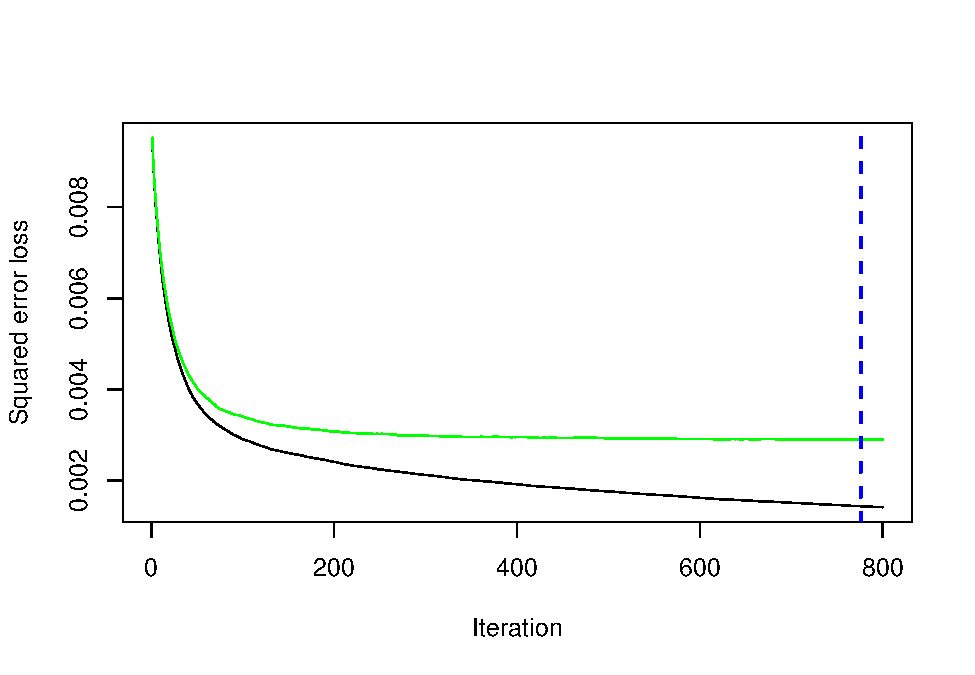
\includegraphics{4271_files/figure-latex/unnamed-chunk-5-1.pdf}

Assignment 1 Bagging Linear Regression: The idea is simple. At each
stage, after bootstrapping the countyElection, build a linear model
(with lm) using all of the available predictors. As before, collect the
predictions at each bootstrap in a matrix (oobPreds). At the end, use
this to compute the error estimate (MSE or Misclassification)

\begin{Shaded}
\begin{Highlighting}[]
\CommentTok{# Linear Model}
\NormalTok{N <-}\StringTok{ }\KeywordTok{nrow}\NormalTok{(countyElection.df)}
\NormalTok{numBoots <-}\StringTok{ }\DecValTok{100}
\NormalTok{oobPreds <-}\StringTok{ }\KeywordTok{matrix}\NormalTok{(}\DataTypeTok{nrow=}\NormalTok{N,}\DataTypeTok{ncol=}\NormalTok{numBoots)}
\ControlFlowTok{for}\NormalTok{(k }\ControlFlowTok{in} \DecValTok{1}\OperatorTok{:}\NormalTok{numBoots)\{}
\NormalTok{  boots <-}\StringTok{ }\KeywordTok{sample}\NormalTok{(}\DecValTok{1}\OperatorTok{:}\NormalTok{N,N,}\DataTypeTok{rep=}\NormalTok{T) }
\NormalTok{  boot.df <-}\StringTok{ }\NormalTok{countyElection.df[boots,]}
\NormalTok{  oobs <-}\StringTok{ }\KeywordTok{setdiff}\NormalTok{(}\DecValTok{1}\OperatorTok{:}\NormalTok{N,boots) }
\NormalTok{  oob.df <-}\StringTok{ }\NormalTok{countyElection.df[oobs,] }
\NormalTok{  bootedTree <-}\StringTok{ }\KeywordTok{lm}\NormalTok{(VoterProp }\OperatorTok{~}\StringTok{ }\NormalTok{.,}
                   \DataTypeTok{data=}\NormalTok{boot.df)}
\NormalTok{  preds <-}\StringTok{ }\KeywordTok{predict}\NormalTok{(bootedTree, }\DataTypeTok{newdata=}\NormalTok{oob.df)}
\NormalTok{  oobPreds[oobs,k] <-}\StringTok{ }\NormalTok{preds }
\NormalTok{\}}
\NormalTok{meanPreds <-}\StringTok{ }\KeywordTok{apply}\NormalTok{(oobPreds,}\DecValTok{1}\NormalTok{,}\ControlFlowTok{function}\NormalTok{(vals) }\KeywordTok{mean}\NormalTok{(vals,}\DataTypeTok{na.rm=}\NormalTok{T))}
\NormalTok{(mse.boots <-}\StringTok{ }\KeywordTok{with}\NormalTok{(countyElection.df, }\KeywordTok{mean}\NormalTok{((meanPreds}\OperatorTok{-}\NormalTok{VoterProp)}\OperatorTok{^}\DecValTok{2}\NormalTok{)))}
\end{Highlighting}
\end{Shaded}

\begin{verbatim}
## [1] 0.00383846
\end{verbatim}

It is quite similar with normal bagging result as we can see above.

Assignment 2 A Random Forest of Linear Regression: The twist now is that
at each stage, select a random subset of the predictors to use. As with
the old Random Forest, establish a mtry to specify how many of the
predictors to select. With these predictors, build a linear model,
predict, etc.

\begin{Shaded}
\begin{Highlighting}[]
\CommentTok{# Linear Model}
\NormalTok{oobPreds <-}\StringTok{ }\KeywordTok{matrix}\NormalTok{(}\DataTypeTok{nrow=}\NormalTok{N,}\DataTypeTok{ncol=}\NormalTok{numBoots) }
\NormalTok{names <-}\StringTok{ }\KeywordTok{names}\NormalTok{(countyElection.df) [}\OperatorTok{-}\KeywordTok{ncol}\NormalTok{(countyElection.df)] }
\NormalTok{numPreds <-}\StringTok{ }\KeywordTok{ncol}\NormalTok{(countyElection.df)}\OperatorTok{-}\DecValTok{1}

\ControlFlowTok{for}\NormalTok{(k }\ControlFlowTok{in} \DecValTok{1}\OperatorTok{:}\NormalTok{numBoots)\{}
\NormalTok{  boots <-}\StringTok{ }\KeywordTok{sample}\NormalTok{(}\DecValTok{1}\OperatorTok{:}\NormalTok{N,N,}\DataTypeTok{rep=}\NormalTok{T)}
\NormalTok{  boot.df <-}\StringTok{ }\NormalTok{countyElection.df[boots,]}
\NormalTok{  oobs <-}\StringTok{ }\KeywordTok{setdiff}\NormalTok{(}\DecValTok{1}\OperatorTok{:}\NormalTok{N,boots)}
\NormalTok{  oob.df <-}\StringTok{ }\NormalTok{countyElection.df[oobs,]}
\NormalTok{  preds <-}\StringTok{ }\KeywordTok{sample}\NormalTok{(}\DecValTok{1}\OperatorTok{:}\NormalTok{numPreds, }\DecValTok{5}\NormalTok{, }\DataTypeTok{rep=}\NormalTok{F)}
\NormalTok{  boot.df <-}\StringTok{ }\NormalTok{boot.df[,}\KeywordTok{c}\NormalTok{(preds, numPreds}\OperatorTok{+}\DecValTok{1}\NormalTok{)] }
\NormalTok{  bootedTree <-}\StringTok{ }\KeywordTok{lm}\NormalTok{(VoterProp }\OperatorTok{~}\StringTok{ }\NormalTok{.,}
                   \DataTypeTok{data=}\NormalTok{boot.df)}
\NormalTok{  preds <-}\StringTok{ }\KeywordTok{predict}\NormalTok{(bootedTree, }\DataTypeTok{newdata=}\NormalTok{oob.df)}
\NormalTok{  oobPreds[oobs,k] <-}\StringTok{ }\NormalTok{preds }
\NormalTok{\}}
\NormalTok{meanPreds <-}\StringTok{ }\KeywordTok{apply}\NormalTok{(oobPreds,}\DecValTok{1}\NormalTok{,}\ControlFlowTok{function}\NormalTok{(vals) }\KeywordTok{mean}\NormalTok{(vals,}\DataTypeTok{na.rm=}\NormalTok{T))}
\NormalTok{(mse.boots <-}\StringTok{ }\KeywordTok{with}\NormalTok{(countyElection.df, }\KeywordTok{mean}\NormalTok{((meanPreds}\OperatorTok{-}\NormalTok{VoterProp)}\OperatorTok{^}\DecValTok{2}\NormalTok{)))}
\end{Highlighting}
\end{Shaded}

\begin{verbatim}
## [1] 0.006475511
\end{verbatim}

It is a bit off comparing with normal random forest result as we can see
above.

Assignment 3 Boosting Linear Regression: Now we go the other direction
with a linear model. At each stage, build a weak linear model consisting
of just one predictor. Select the predictor to use by building a model
for each predictor and select the one that performs best (use MSE or Rˆ2
as a determiner). Use the weak linear model to predict the residuals,
``sand off'' a bit of the predictions using the shrinkage value. Repeat
a bunch of times.

\end{document}
